\documentclass[cs4size,a4paper,nofonts,twoside]{ctexart}
\CTEXsetup[number=\chinese{section}, name={,、}, format={\Large\bfseries}]{section}

\usepackage[utf8]{inputenc}
\def\tjf{{\tt{田劲锋}}}
\def\titlec{《算法设计与分析》综合性实验实验报告}
\usepackage[top=2.54cm,bottom=2.54cm,left=3.17cm,right=3.17cm]{geometry} % 页面设置
\usepackage[unicode,breaklinks=true,
colorlinks=true,linkcolor=black,anchorcolor=black,citecolor=black,urlcolor=black,
pdftitle={\titlec},pdfauthor={\tjf}]{hyperref}
\usepackage{tikz} % 画图
\usetikzlibrary{shapes,arrows}
\usepackage{multicol} % 分栏
\usepackage{multirow} % 跨行
\usepackage{longtable} % 长表格
\usepackage{tabularx} % 变宽表格
\usepackage{booktabs} % 表格画线
\usepackage{graphicx} % 图形
\usepackage{color} % 颜色
\usepackage{xcolor} % 颜色
\usepackage{wallpaper} % 背景图片
\usepackage{listings} % 排版代码
\lstset{language=C++,
  numbers=left,
  numberstyle=\tiny,
  basicstyle=\small\tt,
  commentstyle=\color{gray},
  keywordstyle=\bfseries\color{violet},
  stringstyle=\color{teal},
  showstringspaces=false,
}
\usepackage{amsmath,bm}
\usepackage{verbatim} % 排版代码
\usepackage{url} % 排版链接
\usepackage{shortvrb}
\usepackage{pstricks} % 绘图
\usepackage{pst-tree} % 画树
% \usepackage{pst-uml} % 画 UML
\usepackage{uml} % 画 UML
\usepackage{clrscode3e} % CLRS 伪代码
\usepackage{smartdiagram} % 智能画图
\usepackage{nameref}
\usepackage{rotating} % 横排大图
\usepackage{caption}
\captionsetup{font={small}} % 标题字体大小
\usepackage[inline]{enumitem} % 调整列表样式

%\setmainfont{Times New Roman}
\setCJKmainfont[BoldFont={SimHei}]{SimSun}  % 主要字体:宋体、黑体
\setCJKsansfont[BoldFont={STZhongsong}]{STFangsong} % 次要字体:仿宋、中宋
\setCJKmonofont{KFKai} % 等宽字体:楷体
\setCJKfamilyfont{msyh}[BoldFont={* Bold}]{微软雅黑} \newcommand{\msyh}{\CJKfamily{msyh}} % 微软雅黑
\setCJKfamilyfont{micro}{文泉驿微米黑} \newcommand{\micro}{\CJKfamily{micro}} % 文泉驿微米黑
\setCJKfamilyfont{yaoti}{方正姚体} \newcommand{\yaoti}{\CJKfamily{yaoti}}

\CJKsetecglue{\hspace{0.1em}}
\renewcommand\CJKglue{\hskip -0.3pt plus 0.08\baselineskip}
\frenchspacing
\widowpenalty=10000
\linespread{1.5} % 1.5 倍行距
\setlength{\parskip}{2pt plus 2pt}
\renewcommand{\baselinestretch}{1.5}

\setlength{\abovecaptionskip}{1pt}
\setlength{\belowcaptionskip}{0pt}
\setlength{\intextsep}{8pt}

\makeindex
\pagestyle{plain}


\begin{document}

\newcounter{unit}
\newcommand{\unit}[1]{\stepcounter{unit}\begin{center}\Large\bfseries 实验单元\chinese{unit}\quad #1\end{center}}

\begin{titlepage}

\begin{center}


\includegraphics[height=1cm]{image/haut.png}

\vspace*{1cm}
{\liti\fontsize{48pt}{50pt}{课\quad 程\quad 设\quad 计}}

\vspace*{4cm}
{\fontsize{36}{80}\sf\bfseries \titlec}

\vspace*{1cm}
{\fontsize{30}{70}\sf\bfseries \titlee}

\vfill
{\large
\newcommand{\ctline}[2]{\makebox[6em][s]{\bf #1}:\underline{\makebox[14em][c]{\qquad #2\qquad}}\\}
\ctline{课程设计名称}{数据结构课程设计}
\ctline{专业班级}{计算机 1303 班}
\ctline{学生姓名}{\tjf}
\ctline{学号}{201316920311}
\ctline{指导教师}{白\quad 浩}
\ctline{课程设计时间}{\today}
}

\end{center}

\end{titlepage}

\unit{类和对象}
\section{标准控制台输入输出}
\hfill\ctli{实验时间}{~2014~年~11~月~28~日}

\subsection*{【实验目的】}
\begin{enumerate}[topsep=0pt,partopsep=0pt,itemsep=0pt,parsep=0pt,label={\arabic*、}]
\item 熟悉Dev-Cpp编程环境。
\item 编写简单的输入输出语句。
\item 熟练使用算术运算符。
\item 能够编写简单的判断语句。
\end{enumerate}
\subsection*{【实验环境】}
\MyEnvironment
\subsection*{【实验内容】}
编写C++程序,实现输入两个整数,输出两个整数的加、减、乘、除结果;详细的注释,完整的输出显示。
\subsection*{【详细分析】}
实验内容是简单的对两个输入整数的四则运算,即简单的顺序结构。

在此基础上稍作改动,即输入整数和运算符来自动进行计算,流程如图\ref{aly01}。
\begin{figure}[htp]
\centering
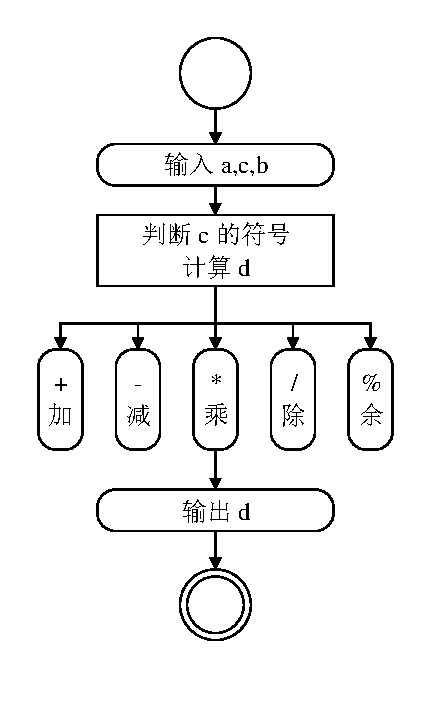
\includegraphics{exp01/exp01.pdf}
\caption{\label{aly01}程序流程图}
\end{figure}
\begin{figure}[htp]
\centering
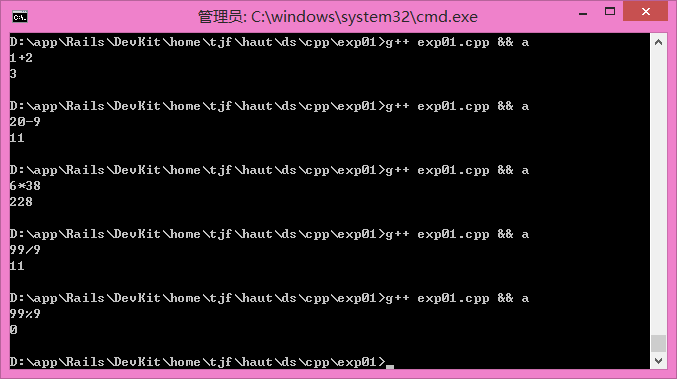
\includegraphics[width=\textwidth]{exp01/exp01.png}
\caption{\label{out01}标准控制台输入输出}
\end{figure}
\subsection*{【实验源码】}
{\linespread{1}\lstinputlisting[caption={\tt exp01.cpp}]{exp01/exp01.cpp}}
\subsection*{【实验结果】}
图\ref{out01}显示了编译、运行、输入、输出的过程。
\subsection*{【实验体会】}
这是一个非常基础的简单程序,目的在于熟悉编程和调试环境。程序本身没有任何难度,加上注释也不过40行。

关于编程环境的配置,我倾向于使用编辑器(如 Vim、Sublime Text)编写源文件,在命令行下编译、运行和调试(使用 gcc/gdb)。当然,Microsoft Visual Studio 作为世界上最好的 IDE ,在编写调试程序中也是非常好用的,所以在有条件的时候也会使用VS。

\clearpage\newpage
 \clearpage
\section{类和对象}
\hfill\ctli{实验时间}{~2014~年~11~月~29~日}
\subsection*{【实验目的】}
\begin{enumerate}[topsep=0pt,partopsep=0pt,itemsep=0pt,parsep=0pt,label={\arabic*、}]
\item 掌握类、对象、数据成员、成员函数的基本概念。
\item 能够进行类的定义。
\item 能够使用成员函数进行相关调用。
\end{enumerate}
\subsection*{【实验环境】}
\MyEnvironment
\subsection*{【实验内容】}
\begin{enumerate}[topsep=0pt,partopsep=0pt,itemsep=0pt,parsep=0pt,label={\arabic*、}]
\item 编写NumberA类,实现两个整数的加减乘除运算。构造函数实现两整数a,b赋值。
\item 编写OperaN类,实现输入1.2.3.4解析成加减乘除符号。
\item P89:3.11
\end{enumerate}

\subsection{NumberA 类}
\subsubsection*{【详细分析】}
NumberA 类设有两个成员变量存放两个操作数,提供对这两个操作数进行四则运算的方法。
\subsubsection*{【实验源码】}
{\linespread{1}\lstinputlisting[caption={\tt exp01.cpp}]{exp02/exp01.cpp}}
\subsubsection*{【实验结果】}
\begin{figure}[htp]
\centering
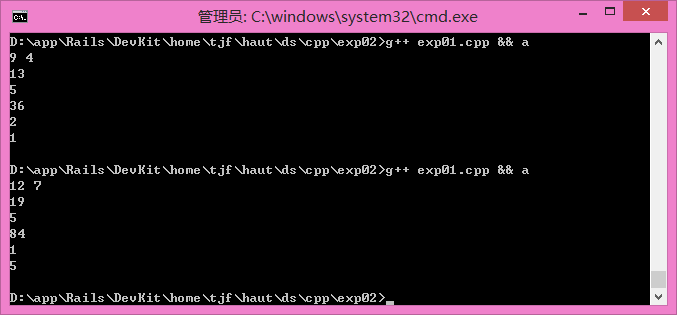
\includegraphics[width=\textwidth]{exp02/exp01.png}
\caption{\label{out02_01}NumberA 类}
\end{figure}

\subsection{OperaN 类}
\subsubsection*{【详细分析】}
用一个整数初始化类,置符号。
\subsubsection*{【实验源码】}
{\linespread{1}\lstinputlisting[caption={\tt exp02.cpp}]{exp02/exp02.cpp}}
\subsubsection*{【实验结果】}
\begin{figure}[htp]
\centering
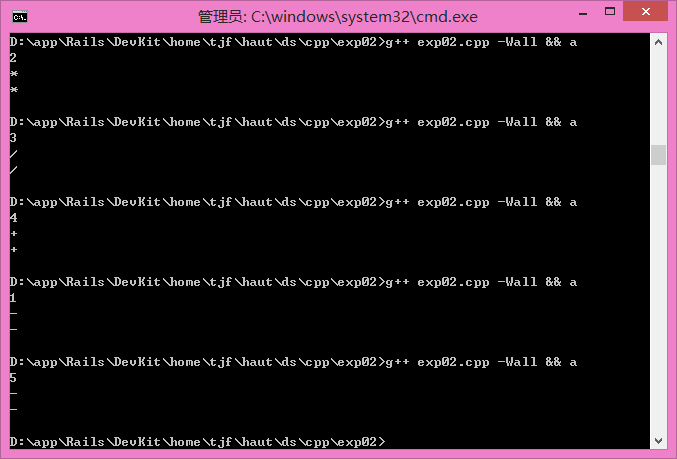
\includegraphics[width=\textwidth]{exp02/exp02.png}
\caption{\label{out02_02}OperaN 类}
\end{figure}

\subsection{P89:3.11}
\subsubsection*{【详细分析】}
对 Account 类的修改。
\subsubsection*{【实验源码】}
{\linespread{1}\lstinputlisting[caption={\tt GradeBook.h}]{exp02/GradeBook.h}}
{\linespread{1}\lstinputlisting[caption={\tt GradeBook.cpp}]{exp02/GradeBook.cpp}}
{\linespread{1}\lstinputlisting[caption={主程序 \tt exp03.cpp}]{exp02/exp03.cpp}}
\subsubsection*{【实验结果】}
\begin{figure}[htp]
\centering
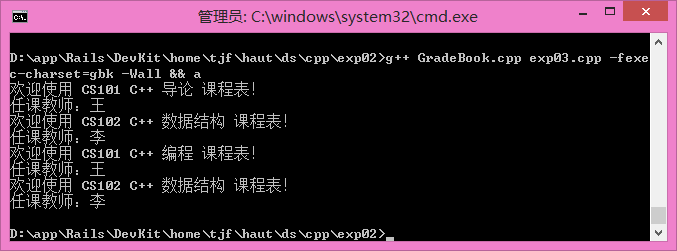
\includegraphics[width=\textwidth]{exp02/exp03.png}
\caption{\label{out02_03}P89:3.11}
\end{figure}

\subsection*{【实验体会】}
(至少150字) \clearpage
\section{结构化控制结构}
\hfill\ctli{实验时间}{~2014~年~11~月~30~日}
\subsection*{【实验目的】}
\begin{enumerate}[topsep=0pt,partopsep=0pt,itemsep=0pt,parsep=0pt,label={\arabic*、}]
\item 掌握基本的结构化控制结构。
\item 能够熟练进行结构化编程。
\end{enumerate}
\subsection*{【实验环境】}
\MyEnvironment
\subsection*{【实验内容】}
\begin{enumerate}[topsep=0pt,partopsep=0pt,itemsep=0pt,parsep=0pt,label={\arabic*、}]
\item 编写NumberA类,实现两个整数的加减乘除运算,可以循环计算。构造函数实现两整数a,b赋值。
\item P177:5.29
\end{enumerate}

\subsection{NumberA 类}
\subsubsection*{【详细分析】}
NumberA 类设有两个成员变量存放两个操作数,提供对这两个操作数进行四则运算的方法。

主程序循环读入两个整数,进行运算并输出。
\subsubsection*{【实验源码】}
{\linespread{1}\lstinputlisting[caption={\tt exp01.cpp}]{exp03/exp01.cpp}}
\subsubsection*{【实验结果】}
\begin{figure}[htp]
\centering
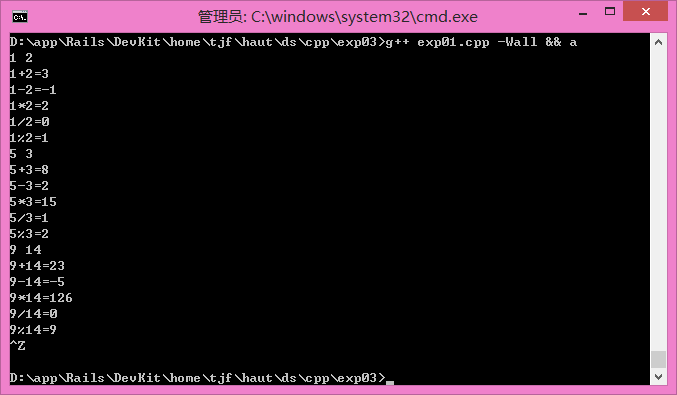
\includegraphics[width=\textwidth]{exp03/exp01.png}
\caption{\label{out03_01}NumberA 类}
\end{figure}

\subsection{P177:5.29}
\subsubsection*{【详细分析】}
用一个整数初始化类,置符号。
\subsubsection*{【实验源码】}
{\linespread{1}\lstinputlisting[caption={\tt exp02.cpp}]{exp02/exp02.cpp}}
\subsubsection*{【实验结果】}
\begin{figure}[htp]
\centering
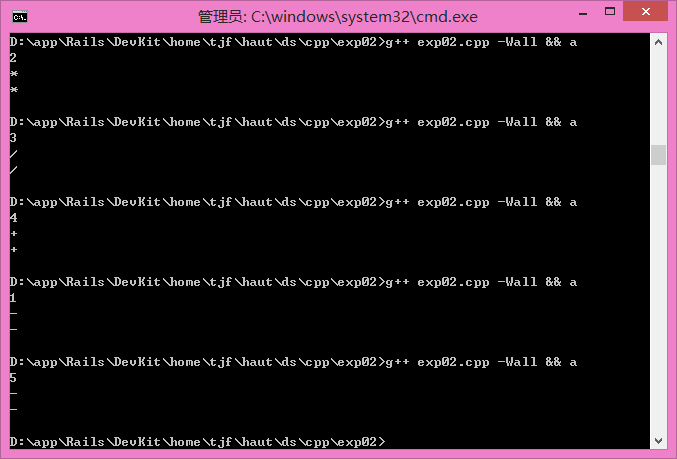
\includegraphics[width=\textwidth]{exp02/exp02.png}
\caption{\label{out03_02}P177:5.29}
\end{figure}

\subsection*{【实验体会】}
(至少150字)
 \cleardoublepage

\begin{titlepage}

\begin{center}


\includegraphics[height=1cm]{image/haut.png}

\vspace*{1cm}
{\liti\fontsize{48pt}{50pt}{课\quad 程\quad 设\quad 计}}

\vspace*{4cm}
{\fontsize{36}{80}\sf\bfseries \titlec}

\vspace*{1cm}
{\fontsize{30}{70}\sf\bfseries \titlee}

\vfill
{\large
\newcommand{\ctline}[2]{\makebox[6em][s]{\bf #1}:\underline{\makebox[14em][c]{\qquad #2\qquad}}\\}
\ctline{课程设计名称}{数据结构课程设计}
\ctline{专业班级}{计算机 1303 班}
\ctline{学生姓名}{\tjf}
\ctline{学号}{201316920311}
\ctline{指导教师}{白\quad 浩}
\ctline{课程设计时间}{\today}
}

\end{center}

\end{titlepage}

\unit{运算符重载}
\section{创建 Date 类}
\hfill\ctli{实验时间}{~2015~年~1~月~8~日}
\subsection*{【实验目的】}
\begin{enumerate}[topsep=0pt,partopsep=0pt,itemsep=0pt,parsep=0pt,label={\arabic*、}]
\item 掌握创建类的方法。
\item 熟悉成员函数的使用方法。
\item 掌握函数和指针的概念
\item 掌握函数和指针的使用方法。
\end{enumerate}
\subsection*{【实验环境】}
\MyEnvironment
\subsection*{【实验内容】}
\begin{enumerate}[topsep=0pt,partopsep=0pt,itemsep=0pt,parsep=0pt,label={\arabic*、}]
\item P89:3.15
\item P348:8.12
\item P354:8.20
\end{enumerate}

\subsection{Date 类}
\subsubsection*{【详细分析】}
创建一个名为 Date 的类,包括了作为数据成员的三部分信息:年月日,都为 int 类型。包括一个具有三个参数的构造函数,用以初始化年月日。假定给出的年、日是正确的,对于不在 1--12 的月,默认设置为 1。对每个数据成员都提供 set/get 函数。提供 displayDate 功能显示格式化后的日期。
\subsubsection*{【实验源码】}
{\linespread{1}\lstinputlisting[caption={\tt Date.h}]{exp04/Date.h}}
{\linespread{1}\lstinputlisting[caption={\tt Date.cpp}]{exp04/Date.cpp}}
{\linespread{1}\lstinputlisting[caption={\tt exp01.cpp}]{exp04/exp01.cpp}}
\subsubsection*{【实验结果】}
\begin{figure}[htp]
\centering
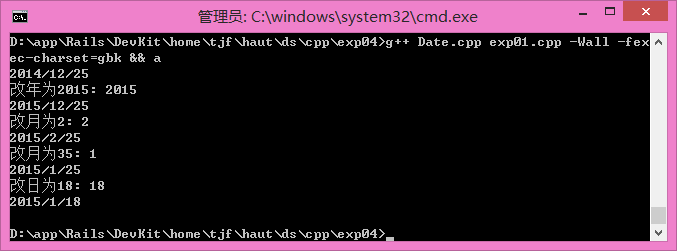
\includegraphics[width=\textwidth]{exp04/exp01.png}
\caption{\label{out04_01}Date 类}
\end{figure}

\subsection{P348:8.12}
\subsubsection*{【详细分析】}
修改课本上的程序,使发牌函数发一手 5 张牌,完成任务:
\begin{enumerate}[topsep=0pt,partopsep=0pt,itemsep=0pt,parsep=0pt,label={\alph*)}]
\item 确定手上是否有一对牌
\item 确定手上是否有两对牌
\item 确定手上是否有 3 张同号牌
\item 确定手上是否有 4 张同号牌
\item 确定手上是否有同花
\item 确定手上是否有顺子
\end{enumerate}

程序对花色和点数分别进行累计,然后循环数出数量。
\subsubsection*{【实验源码】}
{\linespread{1}\lstinputlisting[caption={\tt DeckOfCards.h}]{exp04/DeckOfCards.h}}
{\linespread{1}\lstinputlisting[caption={\tt DeckOfCards.cpp}]{exp04/DeckOfCards.cpp}}
{\linespread{1}\lstinputlisting[caption={\tt exp02.cpp}]{exp04/exp02.cpp}}
\subsubsection*{【实验结果】}
\begin{figure}[htp]
\centering
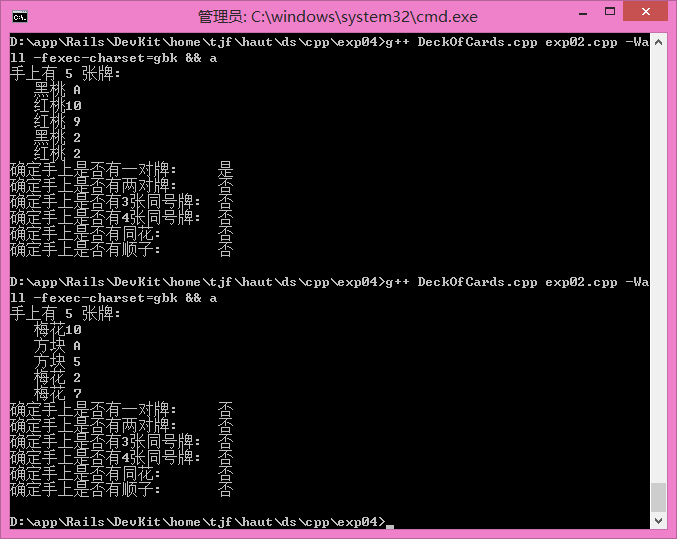
\includegraphics[width=\textwidth]{exp04/exp02.png}
\caption{\label{out04_02}发牌和判断程序}
\end{figure}

\subsection{P354:8.20}
\subsubsection*{【详细分析】}
修改洗牌和发牌程序,使之由同一个函数实现。
\subsubsection*{【实验源码】}
{\linespread{1}\lstinputlisting[caption={\tt DeckOfCards\_plus.cpp}]{exp04/DeckOfCards_plus.cpp}}
{\linespread{1}\lstinputlisting[caption={\tt exp03.cpp}]{exp04/exp03.cpp}}
\subsubsection*{【实验结果】}
\begin{figure}[htp]
\centering
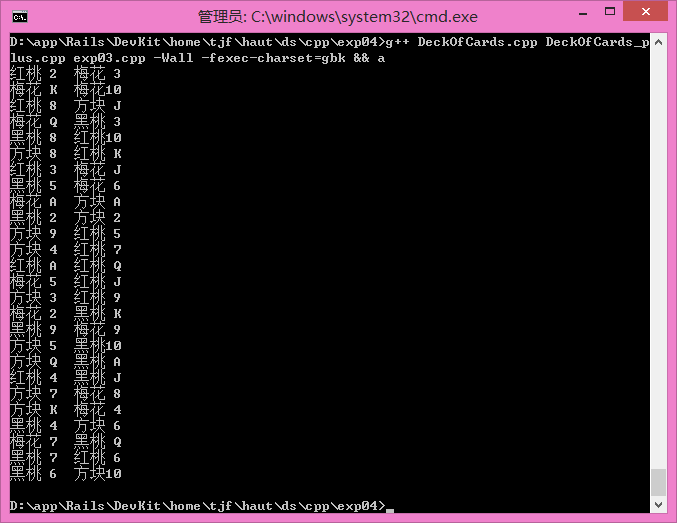
\includegraphics[width=\textwidth]{exp04/exp03.png}
\caption{\label{out04_03}发牌程序}
\end{figure}


\subsection*{【实验体会】}
这次的实验是 Date 类的简单实现,以及对 DeckOfCards 类的修改和增添功能。

对于初始化函数,也就是构造函数,可能会用冒号句法来简化成员对象的赋值。这里因为涉及到特殊判断,所以调用了三个设置函数,而对设置值的特殊处理则分别在设置函数中实现。访问函数有 const 属性,直接返回其值,并不改变值的大小。

判断发牌的花色和点数,则使用了循环查找的暴力算法,由于花色 $n = 4$, 点数 $m = 13$,那么 $O(n)$ 和 $O(m)$ 的算法实际上可以算作常数级别的了。为了简化查找,增设了两个数组来存储花色和点数。函数具有一定的通用性。

最后一个程序删掉了本来的注释,程序显得简练很多了。
 \clearpage
\section{类 Date 的属性}
\hfill\ctli{实验时间}{~2015~年~1~月~9~日}
\subsection*{【实验目的】}
\begin{enumerate}[topsep=0pt,partopsep=0pt,itemsep=0pt,parsep=0pt,label={\arabic*、}]
\item 掌握重载的概念
\item 能够进行运算符重载。
\end{enumerate}
\subsection*{【实验环境】}
\MyEnvironment
\subsection*{【实验内容】}
日期类设计

定义Date类,参照实现:
\begin{enumerate}[topsep=0pt,partopsep=0pt,itemsep=0pt,parsep=0pt,label={(\arabic*)}]
\item 日期的加、减运算
\item 根据日期计算一年中的第几周星期几、一年中第几天为几月几日、该年是否为闰年
\item 输出日期对象
\end{enumerate}

完成相应应用程序设计
\subsection*{【详细分析】}
(此项由学生自己完成)
\subsubsection*{【实验源码】}
{\linespread{1}\lstinputlisting[caption={\tt Date.h}]{exp05/Date.h}}
{\linespread{1}\lstinputlisting[caption={\tt Date.cpp}]{exp05/Date.cpp}}
{\linespread{1}\lstinputlisting[caption={\tt exp01.cpp}]{exp05/exp01.cpp}}
\subsubsection*{【实验结果】}
\begin{figure}[htp]
\centering
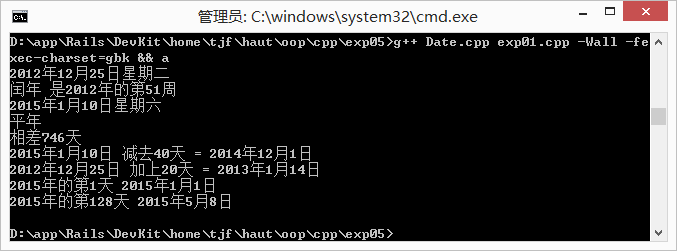
\includegraphics[width=\textwidth]{exp05/exp01.png}
\caption{\label{out05_01}Date 类}
\end{figure}
\subsection*{【实验体会】}
(至少150字)
 \cleardoublepage

\begin{titlepage}

\begin{center}


\includegraphics[height=1cm]{image/haut.png}

\vspace*{1cm}
{\liti\fontsize{48pt}{50pt}{课\quad 程\quad 设\quad 计}}

\vspace*{4cm}
{\fontsize{36}{80}\sf\bfseries \titlec}

\vspace*{1cm}
{\fontsize{30}{70}\sf\bfseries \titlee}

\vfill
{\large
\newcommand{\ctline}[2]{\makebox[6em][s]{\bf #1}:\underline{\makebox[14em][c]{\qquad #2\qquad}}\\}
\ctline{课程设计名称}{数据结构课程设计}
\ctline{专业班级}{计算机 1303 班}
\ctline{学生姓名}{\tjf}
\ctline{学号}{201316920311}
\ctline{指导教师}{白\quad 浩}
\ctline{课程设计时间}{\today}
}

\end{center}

\end{titlepage}

\unit{继承}
\section{创建 Account 继承层次}
\hfill\ctli{实验时间}{~2015~年~1~月~14~日}
\subsection*{【实验目的】}
\begin{enumerate}[topsep=0pt,partopsep=0pt,itemsep=0pt,parsep=0pt,label={\arabic*、}]
\item 掌握继承的概念。
\item 掌握不同继承方式的继承特性。
\end{enumerate}
\subsection*{【实验环境】}
\MyEnvironment
\subsection*{【实验内容】}
P522:12.10
\subsection*{【详细分析】}
创建一个银行账户的继承层次,表示银行的所有客户账户。所有的客户都能在他们的银行账户存钱、取钱,但是账户也可以分成更具体的类型。例如,一方面存款账户 SavingsAccount 依靠存款生利;另一方面,支票账户 CheckingAccount 对每笔交易(即存款或取款)收取费用。

创建一个类层次,以 Account 作为基类,SavingsAccount 和 CheckingAccount 作为派生类。基类 Account 应该包括一个 double 类型的数据成员 balance,表示账户的余额。该类应提供一个构造函数,接受一个初始余额值并用它初始化数据成员 balance。而且构造函数确认初始金额的有效性,保证它大于等于 0。如果小于 0,则需将其置为 0,并显示出错信息,表明该初始化余额是一个无效的值。该类应该提供三个成员函数:成员函数 credit 可以向当前余额加钱;成员函数 debit 负责从账户中取钱,并且保证账户不会透支。如果提取金额大于账户余额,函数将保持 balance 不变,并打印信息“取钱金额超过账户余额”;成员函数 getBalance 则返回当前 balance 的值。

派生类 SavingsAccount 不仅继承了基类 Account 的功能,而且还应提供一个附加的 double 类型数据成员 interestrate 表示这个账户的利率(百分比)。SavingsAccount 的构造函数应接受初始余额值和初始利率值,还应提供一个 pubilc 成员函数 calculateInterest,返回代表账户的利息的一个 double 值,这个值是 balance 和 interestrate 的乘积。注意:类 SavingsAccount 应继承成员函数 credit 和 debit,不需要重新定义。

派生类 CheckingAccount 不仅继承了基类 Account 的功能,还应提供一个附加的 double 类型数据成员 feechargepertransaction 表示每笔交易的费用。CheckingAccount 的构造函数应接受初始金额值和交易费用值。类 CheckingAccount 需要重新定义成员函数 credit 和 debit,当每笔交易完成时,从 balance 中减去 feechargepertransaction。重新定义这些函数时应用到基类 Account 的这两个函数来执行账户余额的更新。CheckingAccount 的 debit 函数只有当钱被成功提取时才应收取交易费。提示:定义 Account 的 debit 函数使它返回一个 bool 类型值,表示钱是否被成功提取。然后利用该值决定是否需要扣除交易费。

当这个层次中的类定义完毕后,编写一个程序,要求创建每个类的对象并测试它们的成员函数。将利息加到 SavingsAccount 对象的方法是:先调用它的成员函数 calculateInterest,然后将返回的利息传递给该对象的 credit 值。

(以上手敲)
\subsection*{【实验源码】}
{\linespread{1}
\lstinputlisting[caption={\tt Account.h}]{exp06/Account.h}
\lstinputlisting[caption={\tt Account.cpp}]{exp06/Account.cpp}
\lstinputlisting[caption={\tt SavingsAccount.h}]{exp06/SavingsAccount.h}
\lstinputlisting[caption={\tt SavingsAccount.cpp}]{exp06/SavingsAccount.cpp}
\lstinputlisting[caption={\tt CheckingAccount.h}]{exp06/CheckingAccount.h}
\lstinputlisting[caption={\tt CheckingAccount.cpp}]{exp06/CheckingAccount.cpp}
\lstinputlisting[caption={\tt exp01.cpp}]{exp06/exp01.cpp}
}
\subsection*{【实验结果】}
\begin{figure}[htp]
\centering
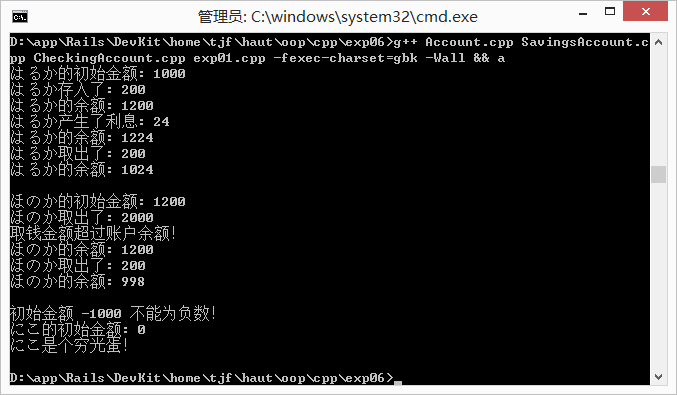
\includegraphics[width=\textwidth]{exp06/exp01.png}
\caption{\label{out06_01}Account 继承层次}
\end{figure}
\subsection*{【实验体会】}
这是一个掌握 C++ 继承的练习题。一个要注意的地方,和其他面向对象语言不同的是,C++ 在父类需要用 virtual 关键字来声明有可能在子类中重载的方法(并且声称这是为了性能)。子类的构造函数中可以调用父类的构造函数,子类的方法也可以调用父类的同名方法。这些特性减少了代码量,避免了代码冗余的产生。这个例子也很好地巩固了继承的概念。
 \cleardoublepage

\begin{titlepage}

\begin{center}


\includegraphics[height=1cm]{image/haut.png}

\vspace*{1cm}
{\liti\fontsize{48pt}{50pt}{课\quad 程\quad 设\quad 计}}

\vspace*{4cm}
{\fontsize{36}{80}\sf\bfseries \titlec}

\vspace*{1cm}
{\fontsize{30}{70}\sf\bfseries \titlee}

\vfill
{\large
\newcommand{\ctline}[2]{\makebox[6em][s]{\bf #1}:\underline{\makebox[14em][c]{\qquad #2\qquad}}\\}
\ctline{课程设计名称}{数据结构课程设计}
\ctline{专业班级}{计算机 1303 班}
\ctline{学生姓名}{\tjf}
\ctline{学号}{201316920311}
\ctline{指导教师}{白\quad 浩}
\ctline{课程设计时间}{\today}
}

\end{center}

\end{titlepage}

\unit{多态性和虚函数}
\section{创建 AHAPE 抽象类}
\hfill\ctli{实验时间}{~2015~年~1~月~14~日}
\subsection*{【实验目的】}
\begin{enumerate}[topsep=0pt,partopsep=0pt,itemsep=0pt,parsep=0pt,label={\arabic*、}]
\item 掌握多态性的概念。
\item 掌握虚函数概念及其与多态性的关系。
\end{enumerate}
\subsection*{【实验环境】}
\MyEnvironment
\subsection*{【实验内容】}
功能要求:

定义一个抽象类SHAPE,抽象方法SHAPE包含X和Y两个属性的访问方法,VOLUME 方法,AREA抽象方法和GETNAME方法。不同的形状类,如POINT 类实现SHAPE 类,RECTANGLE类继承PIONT ,ELLIPSE 类继承RECTANGLE 类。CIRCLE 类继承ELLIPSE 类,CYLINDER类继承CIRCLE类。创建每个类的实例,并将每个类的实例存放于类型为SHAPE的数组中。以该SHAPE的数组作为参数,调用参数的类型为SHAPE 的数组的SHOWSHAPINFO方法,通过调用重写的方法为相应得图形对象计算表面积,体积并输出图形的名称。
\subsection*{【详细分析】}
(此项由学生自己完成)
\subsection*{【实验源码】}
(此项由学生自己完成)
\subsection*{【实验结果】}
(截图给出实验结果)
\subsection*{【实验体会】}
(至少150字)
 \clearpage
% \section{函数和类综合应用}
\hfill\ctli{实验时间}{~2015~年~1~月~15日}
\subsection*{【实验环境】}
\MyEnvironment
\subsection*{【实验内容】}
编写福利彩票双色球的中奖和购买程序

\begin{enumerate}
\item  “双色球”每注投注号码由6个红色球号码和1个蓝色球号码组成。红色球号码从1--33中选择(注意,6个数字各不相同);蓝色球号码从1--16中选择。购买双色球”每注2元。
\item 编写相应的类程序,实现随机生成单注彩票。
\item 初始设置中奖彩票,生成彩票与中奖彩票比对,验证中奖情况,统计奖金和投注数量。
\item 最后显示:
\begin{itemize}[label={}]
\item 中奖:***** 元
\item 投资:***** 元
\item 回报率为:**.** \% (精确显示小数点后两位)
\end{itemize}
\item 提供中断程序的控制,ctrl+z 或者 空格 或者其他
\end{enumerate}

附录为中奖情况:(二等奖固定为200万,一等奖为500万)

\subsection*{【详细分析】}

\subsection*{【实验源码】}
(略)
\subsection*{【实验结果】}
(略)
\subsection*{【实验体会】}
(至少150字)
 \clearpage

\end{document}
